%% Standalone lecture -- build with:  pdflatex -shell-escape gaussianIntegrals
%% Shared preamble for standalone lecture files.
%%
%% Every lecture begins with %% Shared preamble for standalone lecture files.
%%
%% Every lecture begins with %% Shared preamble for standalone lecture files.
%%
%% Every lecture begins with \input{preamble} and is compiled on its own:
%%     pdflatex -shell-escape <lecture>
%% There is no master lectures.tex any more -- the list of lectures lives in
%% lectures.yaml and is read by the build scripts.

\documentclass[25pt,landscape,footrule]{foils}
\input{macros_gen}
\backgroundsetup{contents={}}

\usepackage{stmaryrd}
\usepackage{ifthen}
\usepackage{pdf14}

% Every figure lives in this course's lectures/figures (consolidated
% 2026-10-08).  Do not add other courses' folders back: when a name exists in
% several folders LaTeX silently takes the first, which mixed old and new
% frames of the same animation.  A missing figure should be a build error.
\graphicspath{{figures/}{../lectures/figures/}}

\date{}

\newcounter{lessoncnt}
\newcommand{\lesson}[1]{\setcounter{page}{1}%
\section{Mathematics of Machine Learning\\%
\vfill
\textcolor{red}{\textit{#1}}
\vfill}}
 and is compiled on its own:
%%     pdflatex -shell-escape <lecture>
%% There is no master lectures.tex any more -- the list of lectures lives in
%% lectures.yaml and is read by the build scripts.

\documentclass[25pt,landscape,footrule]{foils}
%\usepackage[compat2,pdftex]{geometry}
\usepackage[pdftex]{geometry}
\geometry{headsep=-2.5ex,hscale=0.9,bmargin=2.5cm,tmargin=1cm,textwidth=25cm}
\usepackage[pdftex]{xcolor}
\usepackage{pause}
\usepackage{background}
%\usepackage[color=white]{background}
\usepackage{listings}
\usepackage{graphicx}
\usepackage{epsfig}
\usepackage{epstopdf}
\usepackage{bm}
\usepackage{amssymb}
\usepackage{amsfonts}
\usepackage{marvosym}
\usepackage{cite}
\usepackage{pifont}
\usepackage[english]{babel}
\usepackage{amsmath}
\usepackage{amsfonts}
\usepackage{rotating}
\usepackage{listings}
\usepackage{pp4slide}
%\usepackage{hyperref}
\usepackage{pp4link}
\usepackage{fancyvrb}
\usepackage{multido}
\usepackage{calc}
\usepackage{mleftright}
\mleftright % Redefines \left to \mleft and \right to \mright



\thinmuskip=1mu

\newcommand{\bigstrut}{\rule[-0.5\baselineskip]{0pt}{1.2\baselineskip}}
\renewcommand{\ttdefault}{pcr}

\newcommand{\squeeze}{\setlength{\itemsep}{-2pt}}
%\renewcommand{\familydefault}{cmr}
%\renewcommand{\labelitemii}{\textcolor{green}{$\star$}}
\newcommand{\tick}{{\large \ding{51}}}
\newcommand{\cross}{{\large \ding{55}}}
%\DeclareMathAlphabet{\mat}{OT1}{cmss}{bx}{n}
\DeclareMathAlphabet{\mat}{U}{eur}{b}{n}
\newcommand{\figs}{/home/apb/figures}
\newcommand{\stimes}{{\scriptstyle \times}}
\newcommand{\tr}{\textsf{T}}
\newcommand{\e}[1]{{\rm e}^{#1}}
\newcommand{\E}[1]{{\rm e}^{{\displaystyle #1}}}
\newcommand{\av}[2][]{\mathbb{E}_{#1}\left[ #2 \right]}
\newcommand{\Var}[1]{\mathbb{V}\mathrm{ar}\left( #1 \right)}
\newcommand{\pred}[1]{\left\llbracket { \small #1} \right\rrbracket}
\newcommand{\logg}[1]{\log\left( #1 \right)}
\newcommand{\logtwo}[1]{\log_2\left( #1 \right)}
\newcommand{\bra}[1]{\left( #1 \right)}
\newcommand{\prob}[1]{\mathbb{P}\left( #1 \right)}
\newcommand{\Prob}[1]{\mathbb{P}\left( #1 \right)}
\newcommand{\Step}{\mathop{\mat{\Theta}}}
\newcommand\diag{\mathop{\mathrm{diag}}}
\newcommand{\grad}{\bm{\nabla}}
\newcommand{\gradx}{\bm{\nabla}_{\!\!\scriptscriptstyle \bm{x}}}
\newcommand{\gradw}{\bm{\nabla}_{\!\!\scriptscriptstyle \bm{w}}}
\newcommand{\dd}{\mathrm{d}}
\newcommand{\ii}{\mathrm{i}}
\newcommand{\data}{\mathcal{D}}
\newcommand{\class}{\mathcal{C}}
\newcommand{\hypo}{\mathcal{H}}
\newcommand{\indep}{\perp \!\!\!\! \perp}
\newcommand{\pd}[3][\,]{\frac{\partial^{#1}{#2}}{\partial\,{#3}}}
\newcommand{\normal}[1]{\mathcal{N}\!\left( #1 \right)}
\newcommand{\Dist}[2][Binom]{\mathrm{#1}\left( \strut {#2} \right)}
\newcommand{\brackets}[1]{\!\left( #1 \right)}
\newcommand{\KL}[2]{\mathop{\mathrm{KL}}\left(#1 \big\| #2\right)}
\newcommand{\argmax}{\mathop{\mathrm{argmax}}}
\newcommand{\argmin}{\mathop{\mathrm{argmin}}}
\newcommand{\margin}{\Delta}
\lstnewenvironment{matlab}[1][frame=TB]{\lstset{#1}}{}       
%\renewcommand{\emph}[1]{\textcolor{red}{\textbf{#1}}}
\newcommand{\myskip}[1]{}
\newcommand\mycom[2]{\genfrac{}{}{0pt}{}{#1}{#2}}
\newcommand{\jl}{\lstinline[basicstyle=\ttfamily\color{DarkGreen},%
 keywordstyle=\bfseries\ttfamily\color{DarkGreen}]}
\definecolor{EmphColor}{rgb}{0.0,0.0,1.0}
\renewcommand{\emph}[1]{{\color{EmphColor}\textbf{#1}}}
\newcommand{\len}[1]{\| #1 \|}
\newcommand{\inner}[2]{\left\langle {#1}, {#2}\right\rangle}
\newenvironment{psmallmatrix}{\left(\begin{smallmatrix}}{\end{smallmatrix}\right)}
  

\definecolor{DarkGreen}{rgb}{0,0.5,0}
\definecolor{DarkRed}{rgb}{0,0,0.5}
\definecolor{HighLight}{rgb}{1,0,0}     % yellow
\definecolor{TextColor}{rgb}{0.0,0.1,0.1}     % white
\definecolor{TwoColor}{rgb}{0.0,0.5,0.1}      % used for switching colors

\definecolor{HeadLineColor}{rgb}{1.0,0.0,0.0} % cyan
\definecolor{SpecialColor}{rgb}{0.53,0.81,1.0}
\renewcommand{\normalcolor}{\color{HeadLineColor}}

\pausecolors{TwoColor}{TextColor}{HighLight}
\pausecolors{EmphColor}{TextColor}{EmphColor}
\pausecolors{DarkGreen}{DarkGreen}{DarkRed}
\pausecolors{SpecialColor}{white}{HighLight}

\newenvironment{PauseHighLight}{\color{TwoColor}\pausehighlight}{}
\newcommand{\multipdf}[2][width=\linewidth]{\multiinclude[pause=\pauselevel{:+0}\pause,format=pdf,graphics={#1}]{#2}}

\lstdefinelanguage{pseudo}
 {keywords={all,and,begin,break,continue,do,else,elseif,%
     end,endif,endfor,endwhile,%
     exit,false,for,forall,goto,if,%
     or,return,then,true,to,repeat,until,while},%
  comment=[s]{/*}{*/},%
  morecomment=[l]//,%
  morestring=[d]"%
 }[keywords,comments,strings]


\lstloadlanguages{Java,pseudo,Python}
\lstset{
  basicstyle=\footnotesize\ttfamily\color{DarkGreen},
  keywordstyle=\bfseries\footnotesize\ttfamily\color{DarkGreen},
  commentstyle=\footnotesize\it\rmfamily\color{blue},
  language=Java,
  showstringspaces=false
  }


\lstnewenvironment{pseudo}[1][]{\lstset{language=pseudo,mathescape,literate={:=}{{$\gets$}}2 {!}{{$\neg$}}1 {!=}{{\!\!$\neq$\,\,}}2 {<=}{{\!\!$\leq$\,\,}}2 {>=}{{\!\!$\geq$\,\,}}2,escapechar=\#,#1}}{}
\lstnewenvironment{java}[1][]{\lstset{escapechar=\$,#1}}{}
% Python code: the language setting makes # comments use commentstyle.
% Comments stay monospaced: the default italic roman letter-spaces badly
% on listings' fixed columns.
\lstnewenvironment{python}[1][frame=TB]{\lstset{language=Python,
    commentstyle=\footnotesize\ttfamily\color{blue},#1}}{}

\MyLogo{}
%\Restriction{}
%\rightfooter{\hyperlink{overview}{$\square$}}

\newcommand{\keywords}[1]{\vfill{\noindent\it #1}}

\newcounter{outlineitem}
\setcounter{outlineitem}{0}
\newcommand{\outlineitem}[2]{\item%
  \def\targ{\value{emumi}}%
  \ifnum\value{enumi}=\value{outlineitem}%
  \color{HighLight}\textbf{#1}\toptarget{#2}\color{TextColor}%
   \else\toplink{#2}{#1}\fi
}
\color{TwoColor}


%-- Instead of writing \section we want the file structured by \section.
\newcommand{\section}[2][0]{\foilhead[#1cm]{#2}}

%-- Write each page into a \begin{slide} -- \end{slide} environment.
\newenvironment{slide}{}{\pauselevel{=1}}

\MyLogo{\pauselevel{=1}\Acrobatmenu{GoBack}{%
  \color{TextColor}{Adam Pr\"ugel-Bennett}} \hspace{2cm}
  % Clicking on the name steps one slide back.
  \toplink{firstoutline}{\color{red}Mathematics of Machine
    Learning}%
  \hspace{2cm}
  \texttt{//ecs-vlc.github.io/aice3001/}
  %Clicking on the date jumps to the last page, which should be the
  %table of contents.
  \rightfooter{\Acrobatmenu{LastPage}{\qquad%
  \textsf{\color{TextColor}\tiny\thepage}}}% page number
  % Clicking on the page number steps one slide back.
}
\raggedright
\newcommand{\Outline}{}

\newcommand{\pb}{\pausebuild \color{TwoColor}}
\newcommand{\pauseb}{\pauselevel{build, highlight}\pause}
\newcommand{\hl}[1]{\pauselevel{=1, highlight =1 :1, highlight =#1 :#1}\pause}
\newcommand{\hll}{\pauselevel{=1, highlight =1 :1}\pause}
\newcommand{\pauseh}{\pauselevel{highlight}\pause}
\newcommand{\nhl}[1]{\textcolor{TextColor}{#1}}
\newcommand{\mypl}[1]{\pauselevel{=#1 :#1}\pause}
\input supp-pdf.tex
\DeclareGraphicsRule{*}{mps}{*}{}
\usepackage{mpmulti}
%\leftheader{}
\rightheader{} % no more page numbers on top right


\hypersetup{pdftitle={ECS Lectures},pdfsubject={Machine Learning}
pdfauthor={Adam Prugel-Bennett},pdfkeywords={machine learning},
pdfpagemode={FullScreen},
bookmarksopen=false,
hypertexnames=false,pdfstartview={FitV},colorlinks,linkcolor={blue},
citecolor={green},urlcolor={blue}}



\newcommand\bluepage{
\clearpage
\renewcommand\normalcolor{\color{yellow}}
\pagecolor{blue}
\renewcommand\Black{\color{white}}
\color{white}
\hypersetup{colorlinks=true}
}

\newcommand\whitepage{
\clearpage
\renewcommand\normalcolor{\color{black}}
\pagecolor{white}
\renewcommand\Black{\color{black}}
\color{black}
\hypersetup{colorlinks=true}
}

\whitepage
\setlength{\unitlength}{1mm}

\newenvironment{leftImage}[2][0.3]{%
\begin{minipage}{#1\linewidth}
  \includegraphics[width=\linewidth]{#2}
\end{minipage}\hfill
\begin{minipage}{0.92\linewidth - #1\linewidth}}%
{\end{minipage}}

\newenvironment{rightImage}[2][0.3]{%
\newcommand{\foot}{\begin{minipage}{#1\linewidth}\includegraphics[width=0.98\linewidth]{#2}\end{minipage}}%
\begin{minipage}{0.95\linewidth - #1\linewidth}\raggedright }{\end{minipage}\hfill\foot}


%%% Local Variables: 
%%% mode: latex
%%% TeX-master: t
%%% End: 

\backgroundsetup{contents={}}

\usepackage{stmaryrd}
\usepackage{ifthen}
\usepackage{pdf14}

% Every figure lives in this course's lectures/figures (consolidated
% 2026-10-08).  Do not add other courses' folders back: when a name exists in
% several folders LaTeX silently takes the first, which mixed old and new
% frames of the same animation.  A missing figure should be a build error.
\graphicspath{{figures/}{../lectures/figures/}}

\date{}

\newcounter{lessoncnt}
\newcommand{\lesson}[1]{\setcounter{page}{1}%
\section{Mathematics of Machine Learning\\%
\vfill
\textcolor{red}{\textit{#1}}
\vfill}}
 and is compiled on its own:
%%     pdflatex -shell-escape <lecture>
%% There is no master lectures.tex any more -- the list of lectures lives in
%% lectures.yaml and is read by the build scripts.

\documentclass[25pt,landscape,footrule]{foils}
%\usepackage[compat2,pdftex]{geometry}
\usepackage[pdftex]{geometry}
\geometry{headsep=-2.5ex,hscale=0.9,bmargin=2.5cm,tmargin=1cm,textwidth=25cm}
\usepackage[pdftex]{xcolor}
\usepackage{pause}
\usepackage{background}
%\usepackage[color=white]{background}
\usepackage{listings}
\usepackage{graphicx}
\usepackage{epsfig}
\usepackage{epstopdf}
\usepackage{bm}
\usepackage{amssymb}
\usepackage{amsfonts}
\usepackage{marvosym}
\usepackage{cite}
\usepackage{pifont}
\usepackage[english]{babel}
\usepackage{amsmath}
\usepackage{amsfonts}
\usepackage{rotating}
\usepackage{listings}
\usepackage{pp4slide}
%\usepackage{hyperref}
\usepackage{pp4link}
\usepackage{fancyvrb}
\usepackage{multido}
\usepackage{calc}
\usepackage{mleftright}
\mleftright % Redefines \left to \mleft and \right to \mright



\thinmuskip=1mu

\newcommand{\bigstrut}{\rule[-0.5\baselineskip]{0pt}{1.2\baselineskip}}
\renewcommand{\ttdefault}{pcr}

\newcommand{\squeeze}{\setlength{\itemsep}{-2pt}}
%\renewcommand{\familydefault}{cmr}
%\renewcommand{\labelitemii}{\textcolor{green}{$\star$}}
\newcommand{\tick}{{\large \ding{51}}}
\newcommand{\cross}{{\large \ding{55}}}
%\DeclareMathAlphabet{\mat}{OT1}{cmss}{bx}{n}
\DeclareMathAlphabet{\mat}{U}{eur}{b}{n}
\newcommand{\figs}{/home/apb/figures}
\newcommand{\stimes}{{\scriptstyle \times}}
\newcommand{\tr}{\textsf{T}}
\newcommand{\e}[1]{{\rm e}^{#1}}
\newcommand{\E}[1]{{\rm e}^{{\displaystyle #1}}}
\newcommand{\av}[2][]{\mathbb{E}_{#1}\left[ #2 \right]}
\newcommand{\Var}[1]{\mathbb{V}\mathrm{ar}\left( #1 \right)}
\newcommand{\pred}[1]{\left\llbracket { \small #1} \right\rrbracket}
\newcommand{\logg}[1]{\log\left( #1 \right)}
\newcommand{\logtwo}[1]{\log_2\left( #1 \right)}
\newcommand{\bra}[1]{\left( #1 \right)}
\newcommand{\prob}[1]{\mathbb{P}\left( #1 \right)}
\newcommand{\Prob}[1]{\mathbb{P}\left( #1 \right)}
\newcommand{\Step}{\mathop{\mat{\Theta}}}
\newcommand\diag{\mathop{\mathrm{diag}}}
\newcommand{\grad}{\bm{\nabla}}
\newcommand{\gradx}{\bm{\nabla}_{\!\!\scriptscriptstyle \bm{x}}}
\newcommand{\gradw}{\bm{\nabla}_{\!\!\scriptscriptstyle \bm{w}}}
\newcommand{\dd}{\mathrm{d}}
\newcommand{\ii}{\mathrm{i}}
\newcommand{\data}{\mathcal{D}}
\newcommand{\class}{\mathcal{C}}
\newcommand{\hypo}{\mathcal{H}}
\newcommand{\indep}{\perp \!\!\!\! \perp}
\newcommand{\pd}[3][\,]{\frac{\partial^{#1}{#2}}{\partial\,{#3}}}
\newcommand{\normal}[1]{\mathcal{N}\!\left( #1 \right)}
\newcommand{\Dist}[2][Binom]{\mathrm{#1}\left( \strut {#2} \right)}
\newcommand{\brackets}[1]{\!\left( #1 \right)}
\newcommand{\KL}[2]{\mathop{\mathrm{KL}}\left(#1 \big\| #2\right)}
\newcommand{\argmax}{\mathop{\mathrm{argmax}}}
\newcommand{\argmin}{\mathop{\mathrm{argmin}}}
\newcommand{\margin}{\Delta}
\lstnewenvironment{matlab}[1][frame=TB]{\lstset{#1}}{}       
%\renewcommand{\emph}[1]{\textcolor{red}{\textbf{#1}}}
\newcommand{\myskip}[1]{}
\newcommand\mycom[2]{\genfrac{}{}{0pt}{}{#1}{#2}}
\newcommand{\jl}{\lstinline[basicstyle=\ttfamily\color{DarkGreen},%
 keywordstyle=\bfseries\ttfamily\color{DarkGreen}]}
\definecolor{EmphColor}{rgb}{0.0,0.0,1.0}
\renewcommand{\emph}[1]{{\color{EmphColor}\textbf{#1}}}
\newcommand{\len}[1]{\| #1 \|}
\newcommand{\inner}[2]{\left\langle {#1}, {#2}\right\rangle}
\newenvironment{psmallmatrix}{\left(\begin{smallmatrix}}{\end{smallmatrix}\right)}
  

\definecolor{DarkGreen}{rgb}{0,0.5,0}
\definecolor{DarkRed}{rgb}{0,0,0.5}
\definecolor{HighLight}{rgb}{1,0,0}     % yellow
\definecolor{TextColor}{rgb}{0.0,0.1,0.1}     % white
\definecolor{TwoColor}{rgb}{0.0,0.5,0.1}      % used for switching colors

\definecolor{HeadLineColor}{rgb}{1.0,0.0,0.0} % cyan
\definecolor{SpecialColor}{rgb}{0.53,0.81,1.0}
\renewcommand{\normalcolor}{\color{HeadLineColor}}

\pausecolors{TwoColor}{TextColor}{HighLight}
\pausecolors{EmphColor}{TextColor}{EmphColor}
\pausecolors{DarkGreen}{DarkGreen}{DarkRed}
\pausecolors{SpecialColor}{white}{HighLight}

\newenvironment{PauseHighLight}{\color{TwoColor}\pausehighlight}{}
\newcommand{\multipdf}[2][width=\linewidth]{\multiinclude[pause=\pauselevel{:+0}\pause,format=pdf,graphics={#1}]{#2}}

\lstdefinelanguage{pseudo}
 {keywords={all,and,begin,break,continue,do,else,elseif,%
     end,endif,endfor,endwhile,%
     exit,false,for,forall,goto,if,%
     or,return,then,true,to,repeat,until,while},%
  comment=[s]{/*}{*/},%
  morecomment=[l]//,%
  morestring=[d]"%
 }[keywords,comments,strings]


\lstloadlanguages{Java,pseudo,Python}
\lstset{
  basicstyle=\footnotesize\ttfamily\color{DarkGreen},
  keywordstyle=\bfseries\footnotesize\ttfamily\color{DarkGreen},
  commentstyle=\footnotesize\it\rmfamily\color{blue},
  language=Java,
  showstringspaces=false
  }


\lstnewenvironment{pseudo}[1][]{\lstset{language=pseudo,mathescape,literate={:=}{{$\gets$}}2 {!}{{$\neg$}}1 {!=}{{\!\!$\neq$\,\,}}2 {<=}{{\!\!$\leq$\,\,}}2 {>=}{{\!\!$\geq$\,\,}}2,escapechar=\#,#1}}{}
\lstnewenvironment{java}[1][]{\lstset{escapechar=\$,#1}}{}
% Python code: the language setting makes # comments use commentstyle.
% Comments stay monospaced: the default italic roman letter-spaces badly
% on listings' fixed columns.
\lstnewenvironment{python}[1][frame=TB]{\lstset{language=Python,
    commentstyle=\footnotesize\ttfamily\color{blue},#1}}{}

\MyLogo{}
%\Restriction{}
%\rightfooter{\hyperlink{overview}{$\square$}}

\newcommand{\keywords}[1]{\vfill{\noindent\it #1}}

\newcounter{outlineitem}
\setcounter{outlineitem}{0}
\newcommand{\outlineitem}[2]{\item%
  \def\targ{\value{emumi}}%
  \ifnum\value{enumi}=\value{outlineitem}%
  \color{HighLight}\textbf{#1}\toptarget{#2}\color{TextColor}%
   \else\toplink{#2}{#1}\fi
}
\color{TwoColor}


%-- Instead of writing \section we want the file structured by \section.
\newcommand{\section}[2][0]{\foilhead[#1cm]{#2}}

%-- Write each page into a \begin{slide} -- \end{slide} environment.
\newenvironment{slide}{}{\pauselevel{=1}}

\MyLogo{\pauselevel{=1}\Acrobatmenu{GoBack}{%
  \color{TextColor}{Adam Pr\"ugel-Bennett}} \hspace{2cm}
  % Clicking on the name steps one slide back.
  \toplink{firstoutline}{\color{red}Mathematics of Machine
    Learning}%
  \hspace{2cm}
  \texttt{//ecs-vlc.github.io/aice3001/}
  %Clicking on the date jumps to the last page, which should be the
  %table of contents.
  \rightfooter{\Acrobatmenu{LastPage}{\qquad%
  \textsf{\color{TextColor}\tiny\thepage}}}% page number
  % Clicking on the page number steps one slide back.
}
\raggedright
\newcommand{\Outline}{}

\newcommand{\pb}{\pausebuild \color{TwoColor}}
\newcommand{\pauseb}{\pauselevel{build, highlight}\pause}
\newcommand{\hl}[1]{\pauselevel{=1, highlight =1 :1, highlight =#1 :#1}\pause}
\newcommand{\hll}{\pauselevel{=1, highlight =1 :1}\pause}
\newcommand{\pauseh}{\pauselevel{highlight}\pause}
\newcommand{\nhl}[1]{\textcolor{TextColor}{#1}}
\newcommand{\mypl}[1]{\pauselevel{=#1 :#1}\pause}
\input supp-pdf.tex
\DeclareGraphicsRule{*}{mps}{*}{}
\usepackage{mpmulti}
%\leftheader{}
\rightheader{} % no more page numbers on top right


\hypersetup{pdftitle={ECS Lectures},pdfsubject={Machine Learning}
pdfauthor={Adam Prugel-Bennett},pdfkeywords={machine learning},
pdfpagemode={FullScreen},
bookmarksopen=false,
hypertexnames=false,pdfstartview={FitV},colorlinks,linkcolor={blue},
citecolor={green},urlcolor={blue}}



\newcommand\bluepage{
\clearpage
\renewcommand\normalcolor{\color{yellow}}
\pagecolor{blue}
\renewcommand\Black{\color{white}}
\color{white}
\hypersetup{colorlinks=true}
}

\newcommand\whitepage{
\clearpage
\renewcommand\normalcolor{\color{black}}
\pagecolor{white}
\renewcommand\Black{\color{black}}
\color{black}
\hypersetup{colorlinks=true}
}

\whitepage
\setlength{\unitlength}{1mm}

\newenvironment{leftImage}[2][0.3]{%
\begin{minipage}{#1\linewidth}
  \includegraphics[width=\linewidth]{#2}
\end{minipage}\hfill
\begin{minipage}{0.92\linewidth - #1\linewidth}}%
{\end{minipage}}

\newenvironment{rightImage}[2][0.3]{%
\newcommand{\foot}{\begin{minipage}{#1\linewidth}\includegraphics[width=0.98\linewidth]{#2}\end{minipage}}%
\begin{minipage}{0.95\linewidth - #1\linewidth}\raggedright }{\end{minipage}\hfill\foot}


%%% Local Variables: 
%%% mode: latex
%%% TeX-master: t
%%% End: 

\backgroundsetup{contents={}}

\usepackage{stmaryrd}
\usepackage{ifthen}
\usepackage{pdf14}

% Every figure lives in this course's lectures/figures (consolidated
% 2026-10-08).  Do not add other courses' folders back: when a name exists in
% several folders LaTeX silently takes the first, which mixed old and new
% frames of the same animation.  A missing figure should be a build error.
\graphicspath{{figures/}{../lectures/figures/}}

\date{}

\newcounter{lessoncnt}
\newcommand{\lesson}[1]{\setcounter{page}{1}%
\section{Mathematics of Machine Learning\\%
\vfill
\textcolor{red}{\textit{#1}}
\vfill}}

% Text that should appear in the animated slides but not in the printable
% (flattened) PDF: near-white there, mapped back to the text colours by ppower4
\definecolor{HandoutHidden}{rgb}{0.999,0.999,0.998}
\pausecolors{HandoutHidden}{TextColor}{HighLight}
% a \pause without the handout marker, for chunks hidden from the handout
\makeatletter
\newcommand{\pausenomark}{\begingroup\pause@nomarkerstrue\pause\endgroup}
\makeatother

\begin{document}

\lesson{Gaussian Integrals}
\vspace{-1cm}
\begin{center}
  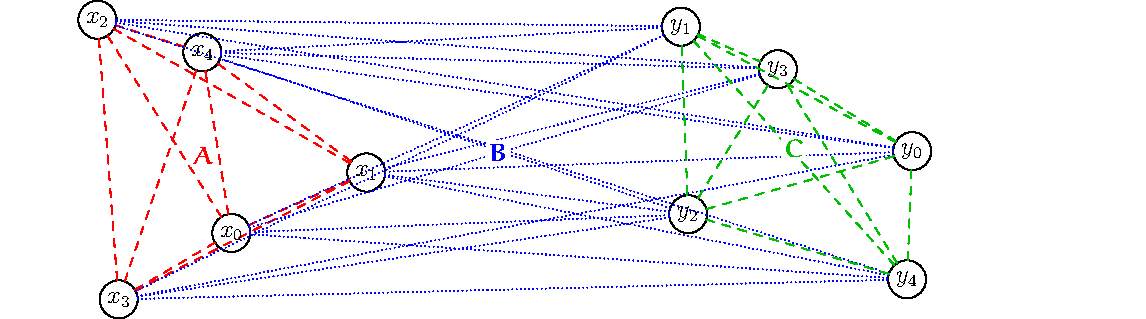
\includegraphics[width=0.6\linewidth]{marginaliseNormals-4}
\end{center}
\keywords{Gaussian integrals, completing the square, moment generating functions, marginals, conditionals, Kalman filter}
%%%%%%%%%%%%%%%%%%%%%%% Next Slide %%%%%%%%%%%%%%%%%%%%%%%
\renewcommand{\Outline}{%
\begin{slide}
\section[1]{Outline}

\begin{minipage}{12cm}\raggedright
  \begin{enumerate}
    \outlineitem{One Dimension}{onedim}
    \outlineitem{Many Dimensions}{manydim}
    \outlineitem{Marginals and Conditionals}{condition}
    \outlineitem{Inference with Gaussians}{inference}
  \end{enumerate}
\end{minipage}\hfill
\begin{minipage}{10cm}
  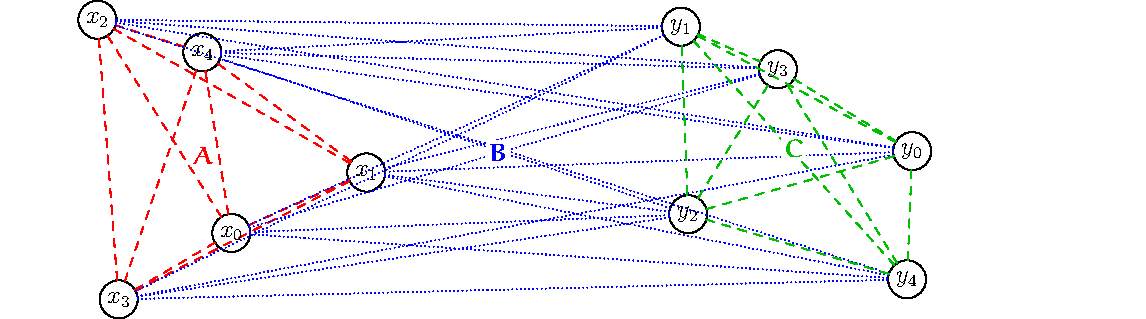
\includegraphics[width=10cm]{marginaliseNormals-4}
\end{minipage}
\end{slide}
\addtocounter{outlineitem}{1}
}

\setcounter{outlineitem}{1}

%%%%%%%%%%%%%%%%%%%%%%% Next Slide %%%%%%%%%%%%%%%%%%%%%%%
\Outline % One Dimension
\toptarget{firstoutline}
%%%%%%%%%%%%%%%%%%%%%%% Next Slide %%%%%%%%%%%%%%%%%%%%%%%

\begin{slide}
\section{Why Gaussians?}

\begin{PauseHighLight}
  \begin{itemize}\squeeze
  \item Gaussians (normal distributions) are everywhere in machine
    learning: Gaussian processes, Kalman filters, linear regression,
    the noise in diffusion models, \ldots\pause
  \item The reason is that we can do all their integrals exactly\pause
  \item Marginalising, conditioning, adding or linearly transforming
    Gaussians gives another Gaussian\pause
  \item The algebra is long-winded, but it uses only three tricks: the
    basic Gaussian integral, completing the square, and diagonalising
    a matrix\pause
  \item Know the results and when to use them; the derivations are
    there so you can trust them\pause
  \end{itemize}
\end{PauseHighLight}

\end{slide}

%%%%%%%%%%%%%%%%%%%%%%% Next Slide %%%%%%%%%%%%%%%%%%%%%%%

\begin{slide}
\section[-2]{The Gaussian Integral}

\begin{PauseHighLight}\squeeze
  \begin{itemize}
  \item We cannot find an antiderivative of $\e{-x^2/2}$, but there is a
    trick: square the integral
    \begin{align*}
      I^2 = \int_{-\infty}^{\infty} \e{-x^2/2}\,\dd x
      \int_{-\infty}^{\infty} \e{-y^2/2}\,\dd y
      = \int_{-\infty}^{\infty}\!\int_{-\infty}^{\infty}
      \e{-(x^2+y^2)/2}\,\dd x\,\dd y\pause
    \end{align*}
  \item In polar coordinates ($x^2+y^2=r^2$, $\dd x\,\dd y =
    r\,\dd r\,\dd\theta$)
    \begin{align*}
      I^2 = \int_0^{2\pi}\dd\theta \int_0^\infty r\,\e{-r^2/2}\,\dd r
      \pause = 2\pi\int_0^\infty \e{-u}\,\dd u \pause = 2\pi
    \end{align*}
    using $u = r^2/2$, $\dd u = r\,\dd r$\pause
  \item So
    \begin{align*}
      \int_{-\infty}^{\infty} \e{-x^2/2}\,\dd x = \sqrt{2\pi}\pause
    \end{align*}
  \end{itemize}
\end{PauseHighLight}

\end{slide}

%%%%%%%%%%%%%%%%%%%%%%% Next Slide %%%%%%%%%%%%%%%%%%%%%%%

\begin{slide}
\section[-2]{Normal Distribution}

\begin{PauseHighLight}
  \begin{itemize}
  \item Changing variables, $z = (x-\mu)/\sigma$ so $\dd x = \sigma\,\dd z$,
    \begin{align*}
      \int_{-\infty}^{\infty} \e{-(x-\mu)^2/(2\sigma^2)}\,\dd x =
      \sigma \int_{-\infty}^{\infty} \e{-z^2/2}\,\dd z =
      \sqrt{2\pi}\,\sigma\pause
    \end{align*}
  \item So the normal density
    \begin{align*}
      \mathcal{N}(x\mid\mu,\sigma^2) = \frac{1}{\sqrt{2\pi}\,\sigma}\,
      \e{-(x-\mu)^2/(2\sigma^2)}
    \end{align*}
    integrates to one\pause
  \item (For small $\sigma$ the density exceeds one at $x=\mu$:
    densities are not probabilities)\pause
  \end{itemize}
\end{PauseHighLight}

\end{slide}

%%%%%%%%%%%%%%%%%%%%%%% Next Slide %%%%%%%%%%%%%%%%%%%%%%%

\begin{slide}
\section[-2]{Completing the Square}

\begin{PauseHighLight}
  \begin{itemize}
  \item Any quadratic in the exponent can be rewritten (for $a>0$)
    \begin{align*}
      -\frac{a}{2}\,x^2 + b\,x = -\frac{a}{2}\left(x - \frac{b}{a}\right)^2
      + \frac{b^2}{2a}\pause
    \end{align*}
  \item So the integral is a shifted Gaussian times a constant
    \begin{align*}
      \int_{-\infty}^{\infty} \e{-\frac{a}{2}x^2 + b\,x}\,\dd x
      = \e{\frac{b^2}{2a}} \int_{-\infty}^{\infty}
      \e{-\frac{a}{2}\left(x - \frac{b}{a}\right)^2}\dd x
      \pause = \sqrt{\frac{2\pi}{a}}\;\e{\frac{b^2}{2a}}\pause
    \end{align*}
  \item This one result does most of the work in this lecture\pause
  \end{itemize}
\end{PauseHighLight}

\end{slide}

%%%%%%%%%%%%%%%%%%%%%%% Next Slide %%%%%%%%%%%%%%%%%%%%%%%

\begin{slide}
\section[-2]{Moment Generating Function}

\begin{PauseHighLight}
  \begin{itemize}
  \item The \emph{moment generating function} of $X$ is
    $M(t) = \av{\e{t\,X}}$\pause
  \item For $X\sim\mathcal{N}(\mu,\sigma^2)$, completing the square gives
    \begin{align*}
      M(t) = \int_{-\infty}^{\infty} \e{t\,x}\,\mathcal{N}(x\mid\mu,\sigma^2)\,\dd x
      = \e{\mu\,t + \frac12\sigma^2 t^2}\pause
    \end{align*}
  \item Expanding $\e{t\,X} = 1 + t\,X + \frac{1}{2}t^2X^2 + \cdots$
    shows $M^{(n)}(0) = \av{X^n}$\pause
    \begin{align*}
      M'(0) = \mu, \qquad M''(0) = \mu^2+\sigma^2\pause
    \end{align*}
  \item The cumulant generating function $\log M(t) = \mu\,t +
    \frac{1}{2}\sigma^2t^2$ stops at $t^2$: a Gaussian has no
    cumulants beyond the mean and variance\pause
  \end{itemize}
\end{PauseHighLight}

\end{slide}

%%%%%%%%%%%%%%%%%%%%%%% Next Slide %%%%%%%%%%%%%%%%%%%%%%%

\begin{slide}
\section[-1]{Sums of Gaussians}

\begin{PauseHighLight}
  \begin{itemize}
  \item A moment generating function determines its distribution\pause
  \item If $X$ and $Y$ are independent,
    $\av{\e{t(X+Y)}} = \av{\e{tX}}\,\av{\e{tY}}$\pause
  \item So for $X\sim\mathcal{N}(\mu_1,\sigma_1^2)$ and
    $Y\sim\mathcal{N}(\mu_2,\sigma_2^2)$
    \begin{align*}
      \av{\e{t(X+Y)}} = \e{(\mu_1+\mu_2)t +
      \frac12(\sigma_1^2+\sigma_2^2)t^2}\pause
    \end{align*}
    which is the MGF of $\mathcal{N}(\mu_1+\mu_2,\,\sigma_1^2+\sigma_2^2)$\pause
  \item Means add and variances add, and the sum is still Gaussian\pause
  \item No integral needed: this is why MGFs are so useful\pause
  \end{itemize}
\end{PauseHighLight}

\end{slide}

%%%%%%%%%%%%%%%%%%%%%%% Next Slide %%%%%%%%%%%%%%%%%%%%%%%
\Outline % Many Dimensions
%%%%%%%%%%%%%%%%%%%%%%% Next Slide %%%%%%%%%%%%%%%%%%%%%%%

\begin{slide}
\section[-2]{Independent Variables}

\begin{PauseHighLight}
  \begin{itemize}
  \item With $\bm{x} = (x_1,\ldots,x_n)^\tr$ and
    $\len{\bm{x}}^2 = \sum_i x_i^2$, the exponential of a sum is a
    product of exponentials
    \begin{align*}
      \int \e{-\frac12\len{\bm{x}}^2}\,\dd\bm{x}
      = \prod_{i=1}^n \int_{-\infty}^{\infty} \e{-x_i^2/2}\,\dd x_i
      = (2\pi)^{n/2}\pause
    \end{align*}
  \item Similarly with a different variance $\lambda_i$ in each
    direction
    \begin{align*}
      \int \e{-\frac12 \sum_i x_i^2/\lambda_i}\,\dd\bm{x}
      = \prod_{i=1}^n \sqrt{2\pi\lambda_i}\pause
    \end{align*}
  \item The general case can be rotated into this one\pause
  \end{itemize}
\end{PauseHighLight}

\end{slide}

%%%%%%%%%%%%%%%%%%%%%%% Next Slide %%%%%%%%%%%%%%%%%%%%%%%

\begin{slide}
\section[-2]{The Multivariate Normal}

\begin{PauseHighLight}\squeeze
  \begin{itemize}
  \item For a positive definite covariance $\mat{\Sigma} =
    \mat{V}\mat{\Lambda}\mat{V}^\tr$ (eigenvalues $\lambda_i>0$) consider
    $I = \int \e{-\frac12(\bm{x}-\bm{\mu})^\tr\mat{\Sigma}^{-1}(\bm{x}-\bm{\mu})}
      \,\dd\bm{x}$\pause
  \item Rotate, $\bm{y} = \mat{V}^\tr(\bm{x}-\bm{\mu})$: the Jacobian
    $\mat{V}$ has $|\det\mat{V}| = 1$ (rotations keep volumes)\pause
    \begin{align*}
      I = \int \e{-\frac12\bm{y}^\tr\mat{\Lambda}^{-1}\bm{y}}\,\dd\bm{y}
      = \prod_i\sqrt{2\pi\lambda_i} = \sqrt{\det(2\pi\mat{\Sigma})}\pause
    \end{align*}
    as $\det\mat{\Sigma} = \prod_i\lambda_i$ and
    $\det(c\,\mat{\Sigma}) = c^n\det\mat{\Sigma}$\pause
  \item So the multivariate normal density is
    \begin{align*}
      \mathcal{N}(\bm{x}\mid\bm{\mu},\mat{\Sigma}) =
      \frac{1}{\sqrt{\det(2\pi\mat{\Sigma})}}\,
      \e{-\frac12(\bm{x}-\bm{\mu})^\tr\mat{\Sigma}^{-1}(\bm{x}-\bm{\mu})}\pause
    \end{align*}
  \end{itemize}
\end{PauseHighLight}

\end{slide}

%%%%%%%%%%%%%%%%%%%%%%% Next Slide %%%%%%%%%%%%%%%%%%%%%%%

\begin{slide}
\section[-2]{Completing the Square in Many Dimensions}

\begin{PauseHighLight}
  \begin{itemize}
  \item For symmetric positive definite $\mat{A}$
    \begin{align*}
      -\frac12\bm{x}^\tr\mat{A}\bm{x} + \bm{b}^\tr\bm{x}
      = -\frac12(\bm{x}-\mat{A}^{-1}\bm{b})^\tr\mat{A}\,
      (\bm{x}-\mat{A}^{-1}\bm{b}) + \frac12\bm{b}^\tr\mat{A}^{-1}\bm{b}\pause
    \end{align*}
    (multiply out the right-hand side to check)\pause
  \item So, by the last slide with $\mat{\Sigma} = \mat{A}^{-1}$,
    \begin{align*}
      \int \e{-\frac12\bm{x}^\tr\mat{A}\bm{x} + \bm{b}^\tr\bm{x}}\,\dd\bm{x}
      = \sqrt{\frac{(2\pi)^n}{\det\mat{A}}}\;
      \e{\frac12\bm{b}^\tr\mat{A}^{-1}\bm{b}}\pause
    \end{align*}
  \item This is the central result: every Gaussian integral in this
    course is an instance of it\pause
  \end{itemize}
\end{PauseHighLight}

\end{slide}

%%%%%%%%%%%%%%%%%%%%%%% Next Slide %%%%%%%%%%%%%%%%%%%%%%%

\begin{slide}
\section[-2]{Multivariate Moment Generating Function}

\begin{PauseHighLight}
  \begin{itemize}
  \item For $\bm{x}\sim\mathcal{N}(\bm{\mu},\mat{\Sigma})$, the central
    result with $\mat{A}=\mat{\Sigma}^{-1}$ gives
    \begin{align*}
      M(\bm{t}) = \av{\e{\bm{t}^\tr\bm{x}}}
      = \e{\bm{t}^\tr\bm{\mu} + \frac12\bm{t}^\tr\mat{\Sigma}\,\bm{t}}\pause
    \end{align*}
  \item Differentiating at $\bm{t}=\bm{0}$
    \begin{align*}
      \av{\bm{x}} = \bm{\mu}, \qquad
      \av{(\bm{x}-\bm{\mu})(\bm{x}-\bm{\mu})^\tr} = \mat{\Sigma}\pause
    \end{align*}
  \item A Gaussian is completely described by its mean and its
    covariance\pause
  \end{itemize}
\end{PauseHighLight}

\end{slide}

%%%%%%%%%%%%%%%%%%%%%%% Next Slide %%%%%%%%%%%%%%%%%%%%%%%

\begin{slide}
\section[-2]{Linear Transformations}

\begin{PauseHighLight}
  \begin{itemize}
  \item Let $\bm{z} = \mat{W}\bm{x} + \bm{c}$ with
    $\bm{x}\sim\mathcal{N}(\bm{\mu},\mat{\Sigma})$\pause
  \item Its MGF is
    \begin{align*}
      \av{\e{\bm{t}^\tr\bm{z}}} = \e{\bm{t}^\tr\bm{c}}\,
      \av{\e{(\mat{W}^\tr\bm{t})^\tr\bm{x}}}\pause
      = \e{\bm{t}^\tr(\mat{W}\bm{\mu}+\bm{c}) +
      \frac12\bm{t}^\tr\mat{W}\mat{\Sigma}\mat{W}^\tr\bm{t}}\pause
    \end{align*}
  \item So
    \begin{align*}
      \bm{z}\sim\mathcal{N}\!\left(\mat{W}\bm{\mu}+\bm{c},\;
      \mat{W}\mat{\Sigma}\mat{W}^\tr\right)\pause
    \end{align*}
  \item Linear maps of Gaussians are Gaussian, and we only need to
    track the mean and covariance\pause{} ($\mat{W}$ need not be
    square)\pause
  \end{itemize}
\end{PauseHighLight}

\end{slide}

%%%%%%%%%%%%%%%%%%%%%%% Next Slide %%%%%%%%%%%%%%%%%%%%%%%
\Outline % Marginals and Conditionals
%%%%%%%%%%%%%%%%%%%%%%% Next Slide %%%%%%%%%%%%%%%%%%%%%%%

\begin{slide}
\section[-2]{Joint Gaussians}

\pause\pb\pauselevel{=1}
\begin{center}
  \multipdf[width=\linewidth]{marginaliseNormals}\pause
\end{center}
% the figure's notation (x, y, A, B, C) while its five frames (levels 1-5)
% are shown, then overwritten in place by the notation used afterwards.
% HandoutHidden keeps the first version out of the printable PDF
\begin{center}
  \pauselevel{=1 :5}\makebox[0pt]{\color{HandoutHidden}$\displaystyle
    \begin{pmatrix}\bm{x}\\ \bm{y}\end{pmatrix} \sim
    \mathcal{N}\!\left(
    \begin{pmatrix}\bm{\mu}^x\\ \bm{\mu}^y\end{pmatrix},
    \begin{pmatrix}\mat{A} & \mat{B}\\
      \mat{B}^\tr & \mat{C}\end{pmatrix}\right)$}\pausenomark
  \pauselevel{=6}\makebox[0pt]{$\displaystyle
    \begin{pmatrix}\bm{z}_1\\ \bm{z}_2\end{pmatrix} \sim
    \mathcal{N}\!\left(
    \begin{pmatrix}\bm{\mu}_1\\ \bm{\mu}_2\end{pmatrix},
    \begin{pmatrix}\mat{\Sigma}_{11} & \mat{\Sigma}_{12}\\
      \mat{\Sigma}_{21} & \mat{\Sigma}_{22}\end{pmatrix}\right),
    \quad \mat{\Sigma}_{21} = \mat{\Sigma}_{12}^\tr$\pause}
\end{center}
\pauselevel{=6}From now on we write $\bm{z}_1$ for $\bm{x}$ and
$\bm{z}_2$ for $\bm{y}$, and $\mat{\Sigma}_{11}$, $\mat{\Sigma}_{12}$
and $\mat{\Sigma}_{22}$ for $\mat{A}$, $\mat{B}$ and $\mat{C}$\pause

\end{slide}

%%%%%%%%%%%%%%%%%%%%%%% Next Slide %%%%%%%%%%%%%%%%%%%%%%%

\begin{slide}
\section[-2]{Marginalising}

\begin{PauseHighLight}
  \begin{itemize}
  \item We want $p(\bm{z}_1) = \int p(\bm{z}_1,\bm{z}_2)\,\dd\bm{z}_2$\pause
  \item Doing the integral directly takes a page of block-matrix
    algebra (see the notes)\pause
  \item Instead take $\bm{t} = (\bm{t}_1, \bm{0})$ in the MGF, so that
    $\bm{t}^\tr\bm{z} = \bm{t}_1^\tr\bm{z}_1$
    \begin{align*}
      \av{\e{\bm{t}_1^\tr\bm{z}_1}} =
      \e{\bm{t}_1^\tr\bm{\mu}_1 + \frac12\bm{t}_1^\tr\mat{\Sigma}_{11}\bm{t}_1}\pause
    \end{align*}
  \item That is the MGF of $\mathcal{N}(\bm{\mu}_1,\mat{\Sigma}_{11})$, so
    \begin{align*}
      \bm{z}_1 \sim \mathcal{N}(\bm{\mu}_1,\mat{\Sigma}_{11})\pause
    \end{align*}
  \item To marginalise, just strike out the rows and columns of the
    variables you integrate away\pause
  \end{itemize}
\end{PauseHighLight}

\end{slide}

%%%%%%%%%%%%%%%%%%%%%%% Next Slide %%%%%%%%%%%%%%%%%%%%%%%

\begin{slide}
\section[-2]{Conditioning: a Light Derivation}

\begin{PauseHighLight}\squeeze
  \begin{itemize}
  \item We want $p(\bm{z}_1\mid\bm{z}_2)$\pause
  \item Subtract the best linear prediction of $\bm{z}_1$ from $\bm{z}_2$
    \begin{align*}
      \bm{w} = \bm{z}_1 - \mat{\Sigma}_{12}\mat{\Sigma}_{22}^{-1}\bm{z}_2\pause
    \end{align*}
  \item $\bm{w}$ is a linear map of $\bm{z}$, so $(\bm{w},\bm{z}_2)$ are
    jointly Gaussian, and
    \begin{align*}
      \mathrm{Cov}(\bm{w},\bm{z}_2) = \mat{\Sigma}_{12} -
      \mat{\Sigma}_{12}\mat{\Sigma}_{22}^{-1}\mat{\Sigma}_{22} = \mat{0}\pause
    \end{align*}
  \item For jointly Gaussian variables, uncorrelated means
    independent\pause{} (the MGF factorises)\pause
  \item So knowing $\bm{z}_2$ tells us nothing about $\bm{w}$, and
    $\bm{z}_1 = \bm{w} + \mat{\Sigma}_{12}\mat{\Sigma}_{22}^{-1}\bm{z}_2$
    with $\bm{z}_2$ now fixed\pause
  \end{itemize}
\end{PauseHighLight}

\end{slide}

%%%%%%%%%%%%%%%%%%%%%%% Next Slide %%%%%%%%%%%%%%%%%%%%%%%

\begin{slide}
\section[-2]{The Conditional Distribution}

\begin{PauseHighLight}
  \begin{itemize}
  \item From the linear-transformation rule, $\bm{w}$ has mean
    $\bm{\mu}_1 - \mat{\Sigma}_{12}\mat{\Sigma}_{22}^{-1}\bm{\mu}_2$ and
    covariance $\mat{\Sigma}_{11} -
    \mat{\Sigma}_{12}\mat{\Sigma}_{22}^{-1}\mat{\Sigma}_{21}$\pause
  \item Hence
    \begin{align*}
      \bm{z}_1\mid\bm{z}_2 \sim \mathcal{N}\!\left(
      \bm{\mu}_1 + \mat{\Sigma}_{12}\mat{\Sigma}_{22}^{-1}(\bm{z}_2-\bm{\mu}_2),\;
      \mat{\Sigma}_{11} - \mat{\Sigma}_{12}\mat{\Sigma}_{22}^{-1}\mat{\Sigma}_{21}
      \right)\pause
    \end{align*}
  \item The mean moves linearly with what we observe\pause
  \item The covariance shrinks, by an amount that does not depend on
    the value we observe\pause
  \item This one formula is the engine behind Gaussian processes and
    Kalman filters\pause
  \end{itemize}
\end{PauseHighLight}

\end{slide}

%%%%%%%%%%%%%%%%%%%%%%% Next Slide %%%%%%%%%%%%%%%%%%%%%%%

\begin{slide}
\section[-2]{The Long Way Round}

\begin{PauseHighLight}
  \begin{itemize}
  \item The same results follow by brute force from the block
    factorisation
    \begin{align*}
      \begin{pmatrix}\mat{\Sigma}_{11} & \mat{\Sigma}_{12}\\
        \mat{\Sigma}_{21} & \mat{\Sigma}_{22}\end{pmatrix}
      = \begin{pmatrix}\mat{I} & \mat{\Sigma}_{12}\mat{\Sigma}_{22}^{-1}\\
        \mat{0} & \mat{I}\end{pmatrix}
      \begin{pmatrix}\mat{S} & \mat{0}\\ \mat{0} & \mat{\Sigma}_{22}\end{pmatrix}
      \begin{pmatrix}\mat{I} & \mat{0}\\
        \mat{\Sigma}_{22}^{-1}\mat{\Sigma}_{21} & \mat{I}\end{pmatrix}\pause
    \end{align*}
    where $\mat{S} = \mat{\Sigma}_{11} -
    \mat{\Sigma}_{12}\mat{\Sigma}_{22}^{-1}\mat{\Sigma}_{21}$ (the
    \emph{Schur complement})\pause
  \item Inverting each factor splits the exponent into a part for
    $\bm{z}_2$ and a part for $\bm{z}_1$ given $\bm{z}_2$\pause
  \item It also gives $\det\mat{\Sigma} = \det\mat{S}\,\det\mat{\Sigma}_{22}$\pause
  \item The full derivation is in the notes: worth reading once, not
    memorising\pause
  \end{itemize}
\end{PauseHighLight}

\end{slide}

%%%%%%%%%%%%%%%%%%%%%%% Next Slide %%%%%%%%%%%%%%%%%%%%%%%
\Outline % Inference with Gaussians
%%%%%%%%%%%%%%%%%%%%%%% Next Slide %%%%%%%%%%%%%%%%%%%%%%%

\begin{slide}
\section[-2]{A Noisy Measurement}

\begin{PauseHighLight}
  \begin{itemize}
  \item Prior belief about a quantity: $x\sim\mathcal{N}(\mu_0, s_0^2)$\pause
  \item We measure $y = x + \epsilon$ with noise
    $\epsilon\sim\mathcal{N}(0,\sigma^2)$\pause
  \item $(x,y)$ is a linear map of $(x,\epsilon)$, so jointly Gaussian with
    \begin{align*}
      \begin{pmatrix} x \\ y\end{pmatrix} \sim
      \mathcal{N}\!\left(\begin{pmatrix}\mu_0\\ \mu_0\end{pmatrix},
      \begin{pmatrix} s_0^2 & s_0^2 \\ s_0^2 & s_0^2+\sigma^2\end{pmatrix}\right)\pause
    \end{align*}
  \item Conditioning on $y$
    \begin{align*}
      \av{x\mid y} = \mu_0 + \frac{s_0^2}{s_0^2+\sigma^2}\,(y-\mu_0),
      \qquad
      \frac{1}{\Var{x\mid y}} = \frac{1}{s_0^2} + \frac{1}{\sigma^2}\pause
    \end{align*}
  \item The estimate moves towards the measurement, and the precisions
    (inverse variances) add\pause
  \end{itemize}
\end{PauseHighLight}

\end{slide}

%%%%%%%%%%%%%%%%%%%%%%% Next Slide %%%%%%%%%%%%%%%%%%%%%%%

\begin{slide}
\section[-1]{Combining Sensors}

\begin{PauseHighLight}
  \begin{itemize}
  \item Two sensors measure the same $x$, with noise variances
    $\sigma_1^2$ and $\sigma_2^2$, giving $y_1$ and $y_2$\pause
  \item With a flat prior ($s_0\to\infty$), applying the last result
    twice gives
    \begin{align*}
      \av{x\mid y_1,y_2} = \frac{y_1/\sigma_1^2 + y_2/\sigma_2^2}
      {1/\sigma_1^2 + 1/\sigma_2^2}, \qquad
      \frac{1}{\Var{x\mid y_1,y_2}} = \frac{1}{\sigma_1^2} +
      \frac{1}{\sigma_2^2}\pause
    \end{align*}
  \item A precision-weighted average: trust the better sensor
    more\pause
  \item With $n$ equally good measurements the variance falls as
    $\sigma^2/n$\pause
  \end{itemize}
\end{PauseHighLight}

\end{slide}

%%%%%%%%%%%%%%%%%%%%%%% Next Slide %%%%%%%%%%%%%%%%%%%%%%%

\begin{slide}
\section[-2]{Predicting One Variable from Another}

\begin{PauseHighLight}
  \begin{itemize}
  \item Two correlated quantities (e.g. height and weight) with
    correlation $\rho$
    \begin{align*}
      \begin{pmatrix} x_1 \\ x_2\end{pmatrix} \sim
      \mathcal{N}\!\left(\begin{pmatrix}\mu_1\\ \mu_2\end{pmatrix},
      \begin{pmatrix} \sigma_1^2 & \rho\,\sigma_1\sigma_2 \\
        \rho\,\sigma_1\sigma_2 & \sigma_2^2\end{pmatrix}\right)\pause
    \end{align*}
  \item Conditioning on $x_1$
    \begin{align*}
      \av{x_2\mid x_1} = \mu_2 + \rho\,\frac{\sigma_2}{\sigma_1}(x_1-\mu_1),
      \qquad
      \Var{x_2\mid x_1} = \sigma_2^2\,(1-\rho^2)\pause
    \end{align*}
  \item The prediction is a straight line: linear regression\pause
  \item As $|\rho|<1$ the prediction is fewer standard deviations from
    the mean than $x_1$ is: \emph{regression to the mean}\pause
  \end{itemize}
\end{PauseHighLight}

\end{slide}

%%%%%%%%%%%%%%%%%%%%%%% Next Slide %%%%%%%%%%%%%%%%%%%%%%%

\begin{slide}
\section[-1]{Tracking: the Kalman Filter}

\begin{PauseHighLight}\squeeze
  \begin{itemize}
  \item A position drifts, $x_{t+1} = x_t + \eta_t$ with
    $\eta_t\sim\mathcal{N}(0,q)$, and is observed as $y_t = x_t +
    \epsilon_t$ with $\epsilon_t\sim\mathcal{N}(0,\sigma^2)$\pause
  \item Our belief stays Gaussian, $x_t\sim\mathcal{N}(m_t, v_t)$.
    \textbf{Predict} (a sum of Gaussians):
    $x_{t+1}\sim\mathcal{N}(m_t,\; v_t + q)$\pause
  \item \textbf{Update:} a noisy measurement, with prior
    $\mathcal{N}(m_t, v_t+q)$
    \begin{align*}
      m_{t+1} &= m_t + k\,(y_{t+1} - m_t), &
      v_{t+1} &= (1-k)(v_t + q),\\
      k &= \frac{v_t+q}{v_t+q+\sigma^2}\pause
    \end{align*}
  \item That is the Kalman filter (with vectors and matrices it guides
    aircraft and phones)\pause
  \end{itemize}
\end{PauseHighLight}

\end{slide}

%%%%%%%%%%%%%%%%%%%%%%% Next Slide %%%%%%%%%%%%%%%%%%%%%%%

\begin{slide}
\section[-2]{Towards Gaussian Processes}

\begin{PauseHighLight}
  \begin{itemize}
  \item Suppose the function values at some inputs are jointly
    Gaussian, and we observe some of them with noise\pause
  \item Put the unknown value $f_*$ in $\bm{z}_1$ and the observations
    $\bm{y}$ in $\bm{z}_2$
    \begin{align*}
      \begin{pmatrix} f_* \\ \bm{y}\end{pmatrix} \sim
      \mathcal{N}\!\left(\bm{0},
      \begin{pmatrix} k_* & \bm{k}_*^\tr \\
        \bm{k}_* & \mat{K}+\sigma^2\mat{I}\end{pmatrix}\right)\pause
    \end{align*}
  \item The conditional formula gives the prediction immediately
    \begin{align*}
      f_*\mid\bm{y} \sim \mathcal{N}\!\left(
      \bm{k}_*^\tr(\mat{K}+\sigma^2\mat{I})^{-1}\bm{y},\;
      k_* - \bm{k}_*^\tr(\mat{K}+\sigma^2\mat{I})^{-1}\bm{k}_*\right)\pause
    \end{align*}
  \item Where the covariances come from is the subject of the next
    lecture\pause
  \end{itemize}
\end{PauseHighLight}

\end{slide}

%%%%%%%%%%%%%%%%%%%%%%% Next Slide %%%%%%%%%%%%%%%%%%%%%%%

\begin{slide}
\section{Summary}

\begin{PauseHighLight}
  \begin{itemize}
  \item The toolkit
    \begin{itemize}
    \item $\int\e{-\frac12\bm{x}^\tr\mat{A}\bm{x}+\bm{b}^\tr\bm{x}}\dd\bm{x}
      = \sqrt{(2\pi)^n/\det\mat{A}}\;\e{\frac12\bm{b}^\tr\mat{A}^{-1}\bm{b}}$\pause
    \item MGF: $\av{\e{\bm{t}^\tr\bm{x}}} =
      \e{\bm{t}^\tr\bm{\mu}+\frac12\bm{t}^\tr\mat{\Sigma}\bm{t}}$\pause
    \item Linear maps: $\mat{W}\bm{x}+\bm{c}\sim
      \mathcal{N}(\mat{W}\bm{\mu}+\bm{c},\mat{W}\mat{\Sigma}\mat{W}^\tr)$\pause
    \item Marginals: strike out rows and columns\pause
    \item Conditionals: $\bm{\mu}_1 +
      \mat{\Sigma}_{12}\mat{\Sigma}_{22}^{-1}(\bm{z}_2-\bm{\mu}_2)$ and
      $\mat{\Sigma}_{11}-\mat{\Sigma}_{12}\mat{\Sigma}_{22}^{-1}\mat{\Sigma}_{21}$\pause
    \end{itemize}
  \item Gaussians stay Gaussian, so inference reduces to linear
    algebra on means and covariances\pause
  \end{itemize}
\end{PauseHighLight}

\end{slide}

\end{document}
